\documentclass[10pt,letter,notitlepage]{article}

\usepackage[left=1.5cm, right=1.5cm, lines=45, top=0.8in, bottom=0.7in]{geometry}
\usepackage{fancyhdr}
\pagestyle{fancy}
\usepackage[most,breakable]{tcolorbox}
\usepackage{xcolor}
\usepackage[linesnumbered,ruled,vlined]{algorithm2e}
\usepackage{amssymb,amsmath}
\usepackage{bm}
\usepackage{dsfont}
\usepackage{enumerate}
\usepackage{enumitem}
\usepackage[normalem]{ulem}
\usepackage{tikz}
\usetikzlibrary{shapes,arrows}
\usepackage{xspace}
\usepackage{lastpage}

\usepackage[breaklinks=true,colorlinks,linkcolor=magenta,urlcolor=magenta,citecolor=black]{hyperref}
\usepackage{cleveref}
\usepackage{xpatch}
\xpretocmd{\algorithm}{\hsize=\linewidth}{}{}

\newtcolorbox[auto counter]{exercise}[1][]{%
	colback=yellow!10,colframe=red!75!black,coltitle=white,use color stack,enforce breakable,enhanced,fonttitle=\bfseries,before upper={\parindent15pt\noindent}, title={\color{white}Exercise~\thetcbcounter: #1}}
\pagecolor{yellow!10}

\lhead{\textbf{University of Waterloo}}
\rhead{\textbf{2022 Fall}}
\chead{\textbf{CS480/680}}
\rfoot{\thepage/\pageref*{LastPage}}
\cfoot{\textbf{Yao-Liang Yu (yaoliang.yu@uwaterloo.ca) \textcopyright 2022}}

\newcommand{\pf}{\mathfrak{p}}
\newcommand{\qf}{\mathfrak{q}}
\newcommand{\pb}{\bar{p}}
\newcommand{\qb}{\bar{q}}
\newcommand{\pfb}{\bar{\mathfrak{p}}}
\newcommand{\qfb}{\bar{\mathfrak{q}}}
\newcommand{\rK}{\reflectbox{\ensuremath{K}}}

\newcommand{\bv}{\mathbf{b}}
\newcommand{\fv}{\mathbf{f}}
\newcommand{\gv}{\mathbf{g}}
\newcommand{\pv}{\mathbf{p}}
\newcommand{\rv}{\mathbf{r}}
\newcommand{\wv}{\mathbf{w}}
\newcommand{\xv}{\mathbf{x}}
\newcommand{\yv}{\mathbf{y}}
\newcommand{\zv}{\mathbf{z}}
\newcommand{\gbs}{\bm{\mathsf{g}}}
\newcommand{\wbs}{\bm{\mathsf{w}}}
\newcommand{\xbs}{\bm{\mathsf{x}}}
\newcommand{\Xv}{\mathbf{X}}
\newcommand{\Yv}{\mathbf{Y}}
\newcommand{\Bsf}{\mathsf{B}}
\newcommand{\Lsf}{\mathsf{L}}
\newcommand{\Xsf}{\mathsf{X}}
\newcommand{\Ysf}{\mathsf{Y}}
\newcommand{\Dc}{\mathcal{D}}
\newcommand{\Nc}{\mathcal{N}}
\newcommand{\EE}{\mathds{E}}
\newcommand{\RR}{\mathds{R}}
\newcommand{\alphav}{\boldsymbol{\alpha}}
\newcommand{\betav}{\boldsymbol{\beta}}
\newcommand{\epsilonv}{\boldsymbol{\epsilon}}
\newcommand{\gammav}{\boldsymbol{\gamma}}

\newcommand{\ans}[1]{{\color{blue}\textsf{Ans}: #1}}
\newcommand{\argmin}{\mathop{\mathrm{argmin}}}
\newcommand{\argmax}{\mathop{\mathrm{argmax}}}
\newcommand{\diag}{\mathrm{diag}}
\newcommand{\dinner}[2]{\langle\!\langle#1,#2\rangle\!\rangle}
\newcommand{\inner}[2]{\langle #1, #2 \rangle}
\newcommand{\one}{\mathbf{1}}
\newcommand{\pred}[1]{[\![#1]\!]}
\newcommand{\prox}[1]{\mathrm{P}_{#1}}
\newcommand{\sgm}{\mathsf{sgm}}
\newcommand{\sign}{\mathop{\mathrm{sign}}}
\newcommand{\tr}{\mathrm{tr}}
\newcommand{\zero}{\mathbf{0}}

\newcommand{\ea}{{et al.}\xspace}
\newcommand{\eg}{{e.g.}\xspace}
\newcommand{\ie}{{i.e.}\xspace}
\newcommand{\iid}{{i.i.d.}\xspace}
\newcommand{\cf}{{cf.}\xspace}
\newcommand{\wrt}{{w.r.t.}\xspace}
\newcommand{\aka}{{a.k.a.}\xspace}
\newcommand{\etc}{{etc.}\xspace}

\newcommand{\red}[1]{{\color{red}#1}}
\newcommand{\blue}[1]{{\color{blue}#1}}
\newcommand{\magenta}[1]{{\color{magenta}#1}}
\newcommand{\green}[1]{{\color{green}#1}}
%===========================================================
\begin{document}
	
	\begin{center}
		\large{\textbf{CS480/680: Introduction to Machine Learning} \\ Homework 2\\ \red{Due: 11:59 pm, November 01, 2022}, \red{submit on LEARN}.} \\
		
		{\bf \green{NAME}} \\
		{\bf \green{student number}}
		
	\end{center}
	
	\begin{center}
		Submit your writeup in pdf and all source code in a zip file (with proper documentation). Write a script for each programming exercise so that the TA can easily run and verify your results. Make sure your code runs!
		
		[Text in square brackets are hints that can be ignored.]
	\end{center}

	\begin{exercise}[Graph Kernels (7 pts)]
		One cool way to construct a new kernel from an existing set of (base) kernels is through graphs. Let $\mathcal{G} = (V, E)$ be a directed acyclic graph (DAG), where $V$ denotes the nodes and $E$ denotes the arcs (directed edges). For convenience let us assume there is a source node $s$ that has no incoming arc and there is a sink node $t$ that has no outgoing arc. We put a base kernel $\kappa_e$ (that is, a function $\kappa_e: \mathcal{X} \times \mathcal{X} \to \mathds{R}$) on each arc $e = (u \to v) \in E$. For each path $P = (u_0 \to u_1 \to \cdots \to u_d)$ with $u_{i-1} \to u_i$ being an arc in $E$, we can define the kernel for the path $P$ as the product of kernels along the path:
		\begin{align}
		\forall \xv, \zv \in \mathcal{X},~
		\kappa_P(\xv, \zv) = \prod_{i=1}^d \kappa_{u_{i-1}\to u_i} (\xv, \zv).
		\end{align}
		Then, we define the kernel for the graph $\mathcal{G}$ as the sum of all possible $s\to t$ \emph{path kernels}:
		\begin{align}
		\forall \xv, \zv \in \mathcal{X},~
		\kappa_{\mathcal{G}}(\xv, \zv) = \sum_{P \in \mathrm{path}(s \to t)} \kappa_P(\xv, \zv).
		\end{align}
		
		\begin{enumerate}
			\item (1 pt) \uline{Prove} that $\kappa_{\mathcal{G}}$ is indeed a kernel. [You may use any property that we learned in class about kernels.]
			
			\ans{\vskip5cm}
			
			\item (1 pt) Let $\kappa_i, i = 1, \ldots, n$ be a set of given kernels. \uline{Construct} a graph $\mathcal{G}$ (with appropriate base kernels) so that the graph kernel $\kappa_{\mathcal{G}} = \sum_{i=1}^n \kappa_i$. Similarly, \uline{construct} a graph $\mathcal{G}$ (with appropriate base kernels) so that the graph kernel $\kappa_{\mathcal{G}} = \prod_{i=1}^n \kappa_i$. 
		
			\ans{\vskip5cm}

			\item (1 pt) Consider the subgragh of the figure below that includes nodes $s, a, b, c$ (and arcs connecting them). \uline{Compute} the graph kernel where $s$ and $c$ play the role of source and sink, respectively. \uline{Repeat the computation} with the subgraph that includes $s, a, b, c, d$ (and arcs connecting them), where $d$ is the sink now.
			
			\begin{center}
				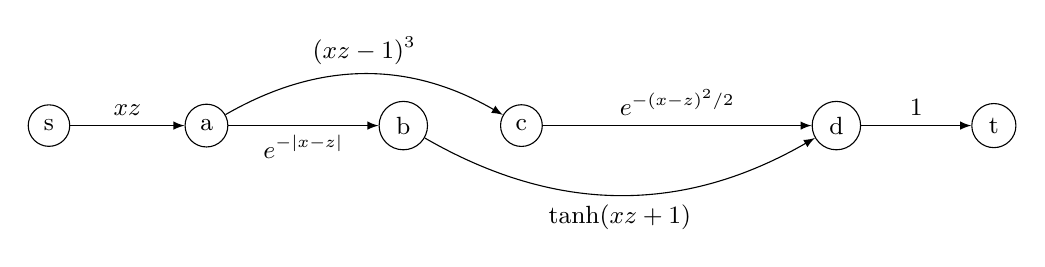
\begin{tikzpicture}[auto]
						\tikzset{align=center,font=\small}
						
						\tikzset{vertex/.style = {shape=circle,draw,minimum size=1.5em}}
						
						\tikzset{edge/.style = {-,> = latex'}}
						
						% vertices
						
						\node[vertex] (s) at  (0,0) {s};
						
						\node[vertex] (a) at  (2,0) {a};
						
						\node[vertex] (b) at  (4.5,0) {b};
						
						\node[vertex] (c) at  (6,0) {c};
						
						\node[vertex] (d) at  (10,0) {d};
						
						\node[vertex] (t) at  (12,0) {t};
						%edges
						
						\begin{scope}[every edge/.style={draw=black,->,> = latex}]
						\draw[edge] (s) edge node{$xz$}  (a);
						\draw[edge] (a) edge node[below] {$e^{-|x-z|}$}  (b);
						\draw[edge] [bend left] (a) edge node {$(xz-1)^3$}  (c);
						\draw[edge] [bend right] (b) edge node[below]{$\tanh(xz+1)$}  (d);
						\draw[edge] (c) edge node{$e^{-(x-z)^2/2}$}  (d);
						\draw[edge] (d) edge node{1}  (t);
						\end{scope}
				\end{tikzpicture}
			\end{center}

			\ans{\vskip3cm}
			
			\item (2 pts) \uline{Find an efficient algorithm to compute the graph kernel} $\kappa_{\mathcal{G}}(\xv, \zv)$ (for two fixed inputs $\xv$ and $\zv$) in time $O(|V| + |E|)$, assuming each base kernel $\kappa_e$ costs $O(1)$ to evaluate. You may assume there is always at least one $s-t$ path. State and justify your algorithm is enough; no need (although you are encouraged) to give a full pseudocode. 
			
			[Note that the total number of paths in a DAG can be exponential in terms of the number of nodes $|V|$, so naive enumeration would not work. For example, replicating the intermediate nodes in the above figure $n$ times creates $2^n$ paths from $s$ to $t$.]
			
			[Hint: Recall that we can use \href{https://en.wikipedia.org/wiki/Topological_sorting}{topological sorting} to rearrange the nodes in a DAG such that all arcs go from a ``smaller'' node to a ``bigger'' one.]
			
			\ans{\vskip5cm}

			\item (2 pts) Let $k: \RR\times \RR \to \RR$ be a kernel whose mixed partial derivative exists:
			\begin{align}
			\frac{\partial^2 k}{\partial s \partial t}(s,t) =: k'(s,t).
			\end{align}
			For example, if $k(s,t) = e^{-\tfrac{1}{2}(s-t)^2}$ is the Gaussian kernel, then the mixed derivative $k'(s,t) = e^{-\tfrac{1}{2}(s-t)^2} [1-(s-t)^2]$.
			
			\uline{Prove} that $k'$ is also a kernel. 
			
			[{\em Hint:} $k'(s, t) = \lim_{\delta s \to0, \delta t\to 0} \frac{k(s+\delta s, t+\delta t) - k(s, t+\delta t) - k(s+\delta s, t) + k( s, t)}{\delta s \cdot \delta t}$.]
			\newpage
			\ans{\vskip9cm}
		\end{enumerate}
	\end{exercise}
	
	
	
	\begin{exercise}[Automatic Differentiation (4 pts)]
		[\blue{\textbf{FYI}: Compare this exercise with the previous one. See any similarity?}]
		
		Recall that in a computational graph $\mathcal{G}$, each node $v$ executes some function $f_v$ on its input nodes $\mathcal{I}_v$ and then sends the output, which we also denote as $v$, i.e. $v = f_v(\mathcal{I}_v)$. Take two arbitrary nodes $u$ and $v$ in $\mathcal{G}$, we claim the following formula:
		\begin{align}
		\label{eq:ad}
		\frac{\partial u}{\partial v} = \sum_{P \in \mbox{path}(v \to u)} \prod_{(v_i, v_{i+1})\in P} 	\frac{\partial v_{i+1}}{\partial v_i},
		\end{align}
		where $\frac{\partial v_{i+1}}{\partial v_i} = \frac{\partial f_{v_{i+1}}}{\partial v_i}$ and by definition node $v_i$ is an input to node $v_{i+1}$.
		
		\begin{enumerate}
			\item (1 pt) \uline{Compute} the following function (i.e., express the sink node $t$ as a function of the source node $s$):
			
			\begin{center}
			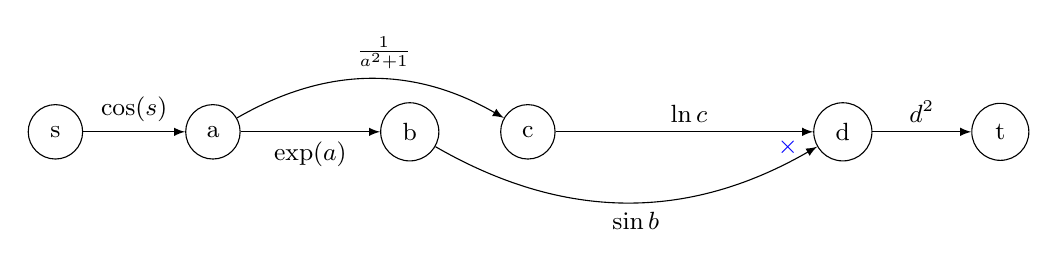
\begin{tikzpicture}[auto]
			\tikzset{text width={width("10")},align=center,font=\small}
			
			\tikzset{vertex/.style = {shape=circle,draw,minimum size=1.5em}}
			
			\tikzset{edge/.style = {-,> = latex'}}
			
			% vertices
			
			\node[vertex] (s) at  (0,0) {s};
			
			\node[vertex] (a) at  (2,0) {a};
			
			\node[vertex] (b) at  (4.5,0) {b};
			
			\node[vertex] (c) at  (6,0) {c};
			
			\node[vertex] (d) at  (10,0) {d};
			
			\node[vertex] (t) at  (12,0) {t};
			%edges
			
			\node (m) at (9.3,-.2) {\blue{$\times$}};
			
			\begin{scope}[every edge/.style={draw=black,->,> = latex}]
			\draw[edge] (s) edge node[text width=2cm] {$\cos(s)$} (a);
			\draw[edge] (a) edge node[below, text width=2cm]{$\exp(a)$}  (b);
			\draw[edge] [bend left] (a) edge node {$\tfrac{1}{a^2+1}$}  (c);
			\draw[edge] [bend right] (b) edge node[below]{$\sin b$}  (d);
			\draw[edge] (c) edge node{$\ln c$}  (d);
			\draw[edge] (d) edge node[text width=2cm]{$d^2$}  (t);
			\end{scope}
			\end{tikzpicture}
			\end{center}
			
			The function implemented by each node is depicted on the \red{incoming} edge. For example, we have $a = \cos s$. For node $d$, we also \blue{multiply} the two incoming edges. 
			
			\ans{\vskip2cm}
			
			\item (1 pt) \uline{Compute} the derivative of $t$ as a function of $s$. You may use the explicit function $t(s)$ that you derived in Ex~2.1.
			
			\ans{\vskip2cm}
			
			\item (1 pt, forward mode) Without loss of generality let us order the nodes as $v_0:=s, v_1=a, v_2 = b, v_3 = c, v_4 = d, t=:v_5$. Going from left to right, and \uline{compute sequentially} 
			\begin{align}
			\frac{\partial v_{i}}{\partial s}, ~~ i = 0, 1, \ldots, 5.
			\end{align}
			For instance $\tfrac{\partial v_0}{\partial s} \equiv 1$. You should not start from scratch for each $i$. Instead, build on results that you have already computed. \uline{Do you need to \href{https://en.wikipedia.org/wiki/Graph_traversal}{traverse} the graph once, twice, or more?} [Hint: your final result $\frac{\partial t}{\partial s}$ should match the one in Ex~2.2, provided that you didn't mess things up in calculus...]
			
			\ans{\vskip1cm
			\begin{align}
			\frac{\partial v_{0}}{\partial s} & = 1 \\
			\frac{\partial v_{1}}{\partial s} & =  \\
			\frac{\partial v_{2}}{\partial s} & =  \\
			\frac{\partial v_{3}}{\partial s} & =  \\
			\frac{\partial v_{4}}{\partial s} & =  \\								
			\frac{\partial t}{\partial s} & =  
			\end{align}
			As shown above, traversing the graph \qquad\qquad is enough to compute $\frac{\partial t}{\partial s}$.
			}
								
			\item (1 pt, backward mode) Similar as above, but this time from right to left and \uline{compute sequentially}
			\begin{align}
			\frac{\partial t}{\partial v_{i}}, ~~ i = 5, 4, \ldots, 0.
			\end{align}
			For instance $\tfrac{\partial t}{\partial v_5} \equiv 1$. You should not start from scratch for each $i$. Instead, build on results that you have already computed. \uline{Do you need to \href{https://en.wikipedia.org/wiki/Graph_traversal}{traverse} the graph once, twice, or more?} [Hint: your final result $\frac{\partial t}{\partial s}$ should match the one in Ex~2.2 and Ex~2.3.]
			
			\ans{\vskip1cm
			\begin{align}
			\frac{\partial t}{\partial v_{5}} & = 1 \\
			\frac{\partial t}{\partial v_{4}} & =  \\
			\frac{\partial t}{\partial v_{3}} & =  \\
			\frac{\partial t}{\partial v_{2}} & =  \\
			\frac{\partial t}{\partial v_{1}} & =  \\								
			\frac{\partial t}{\partial s} & =  
			\end{align}
			
			As shown above, traversing the graph \qquad\qquad is enough to compute $\frac{\partial t}{\partial s}$.
			}
				
		\end{enumerate}
	
	\end{exercise}
	 
	\begin{exercise}[Adaboost (9 pts)]
		In this exercise we will implement Adaboost on a synthetic dataset. Recall that Adaboost aims at minimizing the exponential loss:
		\begin{align}
		\min_{\wv} ~ \sum_i \exp \left( - y_i \sum_j  w_j h_j(\xv_i) \right),
		\end{align}
		where $h_j$ are the so-called weak learners, and the combined classifier 
		\begin{align}
			\label{eq:combined-classifer}
			h_{\wv}(\xv) := \sum_j w_j h_j(\xv). 
		\end{align}
		Note that we \red{assume $y_i \in \{\pm 1\}$} in this exercise, and we \red{simply take $h_j(\xv) = \sign(\pm x_j + b_j)$} for some $b_j \in \RR$. 
		Upon \red{defining $M_{ij} = y_i h_j(\xv_i)$}, we may simplify our problem further as:
		\begin{align}
		\label{eq:adaboost-obj}
		\min_{\wv\in \RR^d} ~ \one^\top \exp(-M\wv),
		\end{align}
		where $\exp$ is applied component-wise and $\one$ is the vector of all 1s.
		
		Recall that $(s)_+ = \max\{s, 0\}$ is the positive part while $(s)_- = \max\{-s, 0\} = |s| - s_+$.
		
		\begin{algorithm}[H]
		\DontPrintSemicolon
			\KwIn{$M\in\RR^{n\times d}$, $\wv_0= \zero_d$, $\pv_0=\one_n$, $\mathsf{max\_pass} = 300$}
			
			\KwOut{$\wv$}
			
			\For{$t=0, 1, 2, \ldots, \mathsf{max\_pass}$ }{
				
				$\pv_t \gets \pv_t / (\one^\top \pv_t)$ \tcp*{normalize}
				
				$\epsilonv_t \gets (M)_-^\top \pv_t $ \tcp*{ $(\cdot)_-$ applied component-wise }
					
				$\gammav_t \gets  (M)_+^\top \pv_t $ \tcp*{$(\cdot)_+$ applied component-wise}
					
				$\betav_{t} \gets \frac12(\ln\gammav_{t} - \ln\epsilonv_t)$ \tcp*{$\ln$ applied component-wise}
				
				choose $\alphav_t \in \RR^d$  \tcp*{decided later}
				
				$\wv_{t+1} \gets \wv_t + \alphav_t \odot \betav_t$  \tcp*{$\odot$ component-wise multiplication}
				
				$\pv_{t+1} \gets \pv_t \odot \exp( - M (\alphav_t \odot \betav_t) ) $  \tcp*{$\exp$ applied component-wise}
			}
			\caption{Adaboost.}
			\label{alg:adaboost}
		\end{algorithm}
		
		\begin{enumerate}
		\item (2 pts) We claim that \Cref{alg:adaboost} is indeed the celebrated Adaboost algorithm if the following holds: 
		\begin{itemize}
		\item $\alphav_t$ is 1 at some entry and 0 everywhere else, i.e., it indicates which weak classifier is chosen at iteration $t$. 
		\item $M \in \{\pm1\}^{n\times d}$, \ie, if all weak classifiers are $\{\pm 1\}$-valued.
		\end{itemize}
		With the above conditions, \uline{prove that (a)} $\gammav_t = \one - \epsilonv_t$, and \uline{(b) the equivalence} between \Cref{alg:adaboost} and the Adaboost algorithm in class. [Note that our labels here are $\{\pm1\}$ and our $\wv$ may have nothing to do with the one in class.]
		
		\ans{\vskip8cm
		}

		\item (3 pts) Let us derive each week learner $h_j$. Consider each feature in turn, we train $d$ linear classifiers that each aims to minimize the weighted training error: 
		\begin{align}
			\min_{b_j\in \RR, s_j \in \{\pm1\}} ~ \sum_{i=1}^n ~ p_i \pred{ y_i (s_j x_{ij} + b_j) \leq 0  },
		\end{align}
		where the weights $p_i \geq 0$ and $\sum_i p_i = 1$. 
		\uline{Find (with justification)} an optimal value for each $b_j$ and $s_j$. [If multiple solutions exist, you can use the middle value.] \uline{Apply} your algorithm to the \href{https://archive.ics.uci.edu/ml/datasets/default+of+credit+card+clients}{default} dataset (available on \href{https://cs.uwaterloo.ca/~y328yu/mycourses/480/assignment.html}{course website}), where $d=23$. \uline{Report} the feature (\ie weak learner) that results in the best and worst test error, respectively, along with its training error. 
		
		\ans{%
		\vskip5cm
		Feature \qquad achieves the best test error at \qquad, with training error \qquad  and $s_j = \qquad , b_j = \qquad $

		Feature \qquad achieves the worst test error at \qquad, with training error \qquad  and $s_j = \qquad , b_j = \qquad $
		}
		
		\item (2 pts) [Parallel Adaboost.] \uline{Implement} \Cref{alg:adaboost} with the following choices: 
		\begin{itemize}
		\item $\alphav_t \equiv \one$
		\item pre-process $M$ by dividing a constant so that for all $i$ (row), $\sum_j |M_{ij}| \leq 1$.
		\end{itemize}
		\uline{Run} your implementation on the \href{https://archive.ics.uci.edu/ml/datasets/default+of+credit+card+clients}{default} dataset (available on \href{https://cs.uwaterloo.ca/~y328yu/mycourses/480/assignment.html}{course website}), and \uline{report the training loss in \eqref{eq:adaboost-obj}, training error, and test error w.r.t. the iteration $t$,} where 
		\begin{align}
			\label{eq:error}
			\mathrm{error}(\wv; \Dc) := \frac{1}{|\Dc|}\sum_{ (\xv, y) \in \Dc} ~\pred{y h_{\wv}(\xv) \leq 0}.
		\end{align}
		[Recall that $h_\wv(\xv)$ is defined in \eqref{eq:combined-classifer} while each $h_j$ is decided in the previous question. In case you fail to determine $h_j$, you may simply use $h_j(\xv) = x_j$ in Ex~2.3 to Ex~2.5.]
		
		[Note that $\wv_t$ is dense (i.e. using all weak classifiers) even after a single iteration.]
		
		\ans{% 
		We report all 3 curves in one figure, with clear coloring and legend to indicate which curve is which.
		\begin{center}
			\includegraphics[width=.5\textwidth]{example-image-a}
		\end{center}
		}
		
		\item (2 pts) [Sequential Adaboost.]  \uline{Implement} \Cref{alg:adaboost} with the following choice: 
		\begin{itemize}
		\item $j_t = \argmax_j | \sqrt{\epsilon_{t,j}} - \sqrt{\gamma_{t,j}} |$ and $\alphav_t$ has 1 on the $j_t$-th entry and 0 everywhere else. 
		%\item pre-process $M$ by dividing a constant so that for all $i$ and $j$, $|M_{ij}| \leq 1$.
		\end{itemize}
		\uline{Run} your implementation on the \href{https://archive.ics.uci.edu/ml/datasets/default+of+credit+card+clients}{default} dataset (available on \href{https://cs.uwaterloo.ca/~y328yu/mycourses/480/assignment.html}{course website}), and \uline{report the training loss in \eqref{eq:adaboost-obj}, training error, and test error in \eqref{eq:error} w.r.t. the iteration $t$.}
		
		[Note that $\wv_t$ has at most $t$ nonzeros (i.e. weak classifiers) after $t$ iterations.]
		
		\ans{%		
		We report all 3 curves in one figure, with clear coloring and legend to indicate which curve is which.
		\begin{center}
			\includegraphics[width=.5\textwidth]{example-image-b}
		\end{center}
		}

		\end{enumerate}
	\end{exercise}

\end{document}
              